% !TEX = root../thesis.tex

\chapter{Real Time Muon Reconstruction at the Compact Muon Solenoid}
\label{chap:kbmtf}

\section{Introduction} \label{sec:kbmtf_intro}
Section~\ref{sec:CMS_L1T} provides an overview of the L1 trigger and its importance to the CMS trigger system. This section will detail the design and performance of a Kalman Filter algorithm used to identify muon tracks in the barrel region of the CMS detector. This algorithm, known as the Kalman Barrel Muon Track Finder (KBMTF), was fully implemented for 2018 data taking and received improvements for continued use in Run-3.

\section{The Kalman Filter Algorithm} \label{sec:kalman_filter}
A Kalman Filter is a tracking algorithm that effectively performs a recursive, iterative chi-squared fit. Qualitatively, it propagates a system from its current state to the next and combines the predicted value with measurements to "update" the state of the system. This updated system can then be propagated and combined with new measured values. This section deals specifically with a discrete linear Kalman Filter, which is applicable when a system can be described with a vector of variables whose evolution can be modeled with a linear transformation plus random uncertainties~\cite{FRUHWIRTH1987444}.

Abstractly, the state of a system at a given step $n-1$ can be described by a vector labeled $x_{n-1}$ with covariance matrix $P_{n-1}$. Let the matrix $F_n$ represent the linear transformation that propagates $x_{n-1}$ to the next state $x_{n}$, and the matrix $Q_{n}$ be the covariance matrix due to random uncertainty. The predicted state of the system at step $n$ can be given by
\begin{equation}
	\label{eq:prop}
	x_{n}=F_{n}x_{n-1} \quad \textrm{and} \quad P_{n}=F_nP_{n-1}F_n^T+Q_n
\end{equation}

Now define a set of measurements taken at state $n$ as $z_n$ with covariance matrix $R_n$. The measured variables are not restricted to the same set of variables defining $x_n$ as long as there exist a change of basis matrix $H$ that relates the sets. The predicted state and covariance matrix of the system written in the same basis as the measured quantities is defined as
\begin{equation}
	\label{eq:changeOfBasis}
	\mu_n\coloneqq Hx_n \quad \textrm{and} \quad \Sigma_n\coloneqq HP_nH^{T}
\end{equation}

Updating the system relies on a matrix known as the Kalman Gain, which acts as a weight based on $\Sigma_n$ and $R_n$ and effectively determines if the updated system should skew more towards the measured or predicted values. The Kalman gain is defined as
\begin{equation}
	\label{eq:gain}
	K\coloneqq \Sigma_n\left(\Sigma_n+R_n\right)^{-1}
\end{equation}

The Kalman gain is then used to calculate the updated system as follows
\begin{equation}
	\label{eq:update1}
	\mu_n'=\mu_n+K\left(z_n-\mu_n\right) \quad \textrm{and} \quad \Sigma_n'=\Sigma_n-K\Sigma_n
\end{equation}

Elements in term $z_n-\mu_n$ are frequently referred to as the residuals. A kalman gain equal to the identity $I$ would set the updated coordinates to the measured values, while a kalman gain of $0$ would effectively ignore the measured values. Finally, we substitute $\mu$ and $\Sigma$ using equation~\ref{eq:changeOfBasis} and simplify to give
\begin{equation}
	x_n'=x_n+K'(z_n-Hx_n) \quad \mathrm{and} \quad P_n'= P_n-K'HP_n
\end{equation}
where the Kalman Gain $K$ has been redefined to
\begin{equation} \label{eq:gain2}
	K'=P_nH^T(HP_nH^T+R_n)^{-1}
\end{equation}
The system $x_n'$ and $P_n'$ can now be propagated to step $n+1$ where the Kalman Algorithm can be repeated.

\section{The Kalman Barrel Muon Track Finder} \label{sec:kbmtf}
Muon track finding begins from the outer chambers and propagates inward because the outermost chambers are the lowest occupancy, as background events are more likely to be stopped as they travel through more material. A rough outline KBMTF algorithm for track finding is as follows:
\begin{enumerate}
	\item A track seed is chosen from stubs in the muon station, which provides a preliminary track with $k$, $\phi$, and $\phi_{b}$. This seed cannot be chosen from the innermost muon station.
	\item If the track is not at the innermost station, the track is propagated inward to the next station. \label{kbmtf_step2}
	\item Stubs in the inner station are matched to the propagated track. \label{kbmtf_step3}
	\begin{itemize}
		\item If there is a matching stub, create an updated track using the stub information
	\end{itemize}
	\item Repeat steps~\ref{kbmtf_step2}-\ref{kbmtf_step3} until the track is at the innermost station
	\item Propagate the track from the innermost station to the vertex
	\begin{itemize}
		\item The $d_{xy}$ of the track is defined as the closest distance from this propagated track to the vertex, and the track values are stored as the "vertex unconstrained" measurement.
	\end{itemize} \label{kbmtf_step4}
	\item The vertex propagated track is updated with the constraint that the track originated from the beamline, known as the "vertex constrained" measurement. \label{kbmtf_step5}
\end{enumerate}

Tracks are then overlap cleaned, which ensures that stubs are not shared between multiple tracks, and cut based on various goodness of fit criteria. A diagram showing the KBMTF propagation and update procedure can be shown in figure~\ref{fig:kbmtf}.

\begin{figure} [htb!]
	\centering
	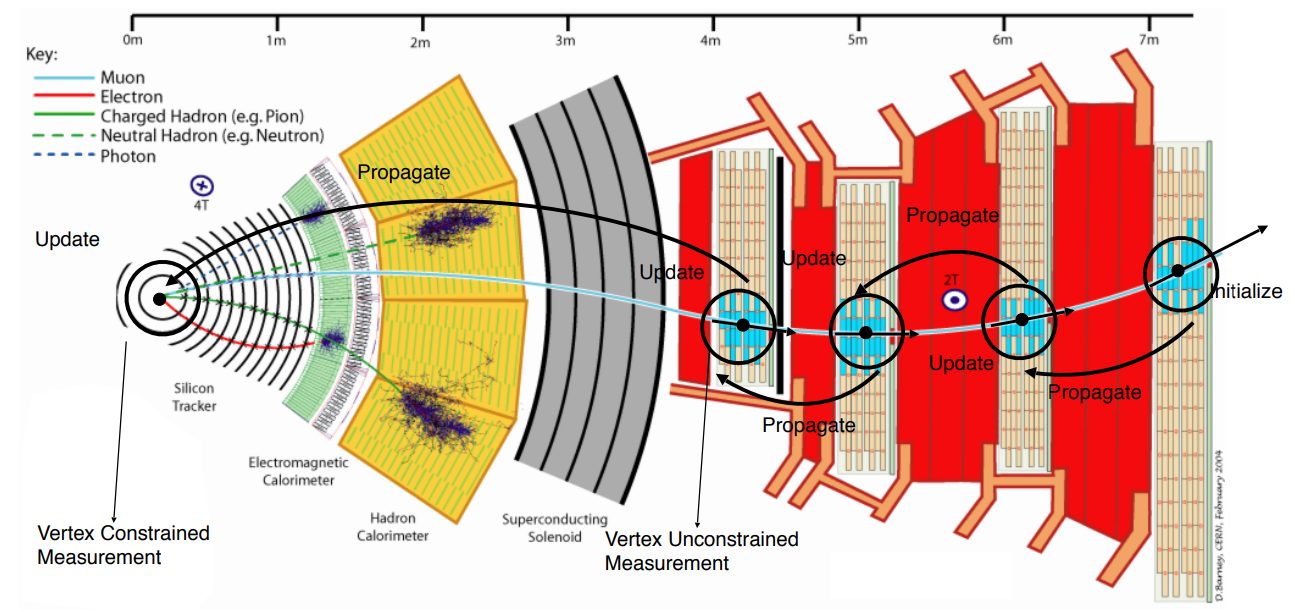
\includegraphics[width=0.85\linewidth]{figs/04_muons/kbmtf_diagram.png}
	\caption[The iterative process of propagation and updating a muon track through the KBMTF algorithm. The track properties at the innermost station are stored in order to trigger on muons not originating from the beamline~\cite{CERN-LHCC-2020-004}]
	{The iterative process of propagation and updating a muon track through the KBMTF algorithm. The track properties at the innermost station are stored in order to trigger on muons not originating from the beamline~\cite{CERN-LHCC-2020-004}.}
	\label{fig:kbmtf}
\end{figure}

\subsection{Muon Trajectory Propagation} \label{sec:muons_prop}
In order to implement a Kalman Filter, the propagation of muon tracks between stations must be expressed as a linear function of $k$, $\phi$, and $\phi_b$. The passage of charged particles through magnetic fields is well understood from the Lorentz Force Law. Using the geometry described in section~\ref{sec:CMS_coord}, a particle with charge $q$ and transverse momentum $p_T$ travels in a circular trajectory with radius $R$ when viewed in the $r$-$\varphi$ plane. These can be related by $p_{T} = qBR$. In particle physics, when working with an object of elementary charge, this is commonly rewritten as
\begin{equation}
	\label{eq:pt03br}
	p_{T} = 0.3BR\unit{[GeV/c]}
\end{equation} 

With the high center of mass energy, the radius of these trajectories is substantially larger than the size of the CMS detector. Assuming a coordinate system with the particle starting at the origin, the circular trajectory can be approximated using a parabola as
\begin{equation}
	\label{eq:parabola1}
	y(x)=\frac{x^2}{2R}+bx
\end{equation}
where $b$ is a coefficient depending on the orientation of the coordinate system. If the initial trajectory is defined as $\phi_{b,0}$, taking the derivative and evaluating at the origin yields
\begin{equation}
	\label{eq:phib}
	y'(0)=\tan(\phi_{b,0})=b
\end{equation}	
The curvature $k=q/p_{T}$, where the muon charge $q=\pm1$, is the preferred variable to work with when propagating the trajectory of a muon, as the propagation is linear in $k$. This along with equations~\ref{eq:pt03br}-\ref{eq:phib}, and combining constant coefficients of x, yields
\begin{equation}
	\label{eq:parabola2}
	y(x)=akx^2+\tan(\phi_{b,0})x
\end{equation}

Muon hits (or "stubs") provide information on the position $\phi$ and bending angle $\phi_b$. Let the radius of two sequential muon stations as $r_1$ and $r_2$, with the outer radius given by $r_2$ and $\Delta r=r_2-r_1$. Assuming a muon has curvature $k$ at the outer station and negligible energy loss, equation~\ref{eq:parabola2} can be used to propagate stubs from the outer station towards the inner station.
\begin{equation}
	y(-\Delta r) = \left(a\Delta r^2\right)k-\Delta r\tan(\phi_{b,0})
\end{equation}
\begin{equation}
	y'(-\Delta r)=-\left(2a\Delta r\right)k+\tan(\phi_{b,0})
\end{equation}
Converting these to the quantities to angles yields
\begin{equation}
	\label{eq:prop_phi}
	\sin(\Delta\phi)\approx\Delta\phi=\frac{y(-\Delta r)}{r_1} = \frac{a\Delta r^2}{r_1}k-\frac{\Delta r}{r_1}\phi_{b,0}
\end{equation}
\begin{equation}
	\label{eq:prop_phib}
	\phi_b=\Delta\phi+\mathrm{tan}^{-1}\left[y'(-\Delta r)\right]\approx a\Delta r\left(\frac{\Delta r}{r_1}-2\right)k+\left(\frac{r_2}{r_1}\right)\phi_{b,0}
\end{equation}
Where we have used the small angle approximation to simplify $\sin(x)$, $\tan(x)$, and $\mathrm{tan}^{-1}(x)$ as $\sim x$ in order to express the propagated coordinates as a linear combination of the initial curvature $k$, position $\phi$, and bending angle $\phi_{b,0}$. The $\Delta\phi$ term is added to equation~\ref{eq:prop_phib} because the bending angle at each station is measured relative to an axis system oriented towards the center of the detector. A diagram showing this propagation can be seen in figure~\ref{fig:mu_trajectory}.

\begin{figure}[h!]
	\centering
	%Final image: origin at outer stub, oriented with x axis pointing towards vertex
	\begin{tikzpicture}
		% axis system
		\draw[thick,->] (-11, 0) -- (1, 0) node[anchor=west] {x};
		\draw[thick,->] (0, 0) -- (0, 4) node[anchor=south east] {y};
		\coordinate[label = above left:$\mathrm{Vertex}$] (vertex) at (-9.5, 0);
		\coordinate[label = above right:$\mathrm{Origin}$] (origin) at (0, 0);
		\coordinate[] (r1) at (-5, 0);
		\node at (vertex)[circle,fill,inner sep=2pt]{};
		\node at (origin)[circle,fill,inner sep=2pt]{};
		\draw[<->] (-9.5, -.5) -- (-5, -.5);
		\draw[<->] (-9.5, -1.1) -- (0, -1.1);
		\coordinate[label = below:$r_1$] (r1) at (-7.25,-.5);
		\coordinate[label = below:$r_2$] (r2) at (-5,-1.1);
		\draw[dashed] (-5, 0) -- (-5, 4);
		
		% muon trajectory
		\def \X{2.6047227}; %circle x0
		\def \Y{14.772116}; %circle y0
		
		\def \sy{1.8427620};%stub at (-5, y)
		\draw [<-, domain=270:230] plot ({\X+15*cos(\x)}, {\Y+15*sin(\x)});
		\draw (-2.25,.25) node[anchor=west] {$\phi_{b,0}$};
		\coordinate[] (stub1) at (-5, \sy);
		\draw [dashed, domain=0:6] plot ({-9.5+\x}, {0.40950267*\x});
		\draw [dashed] (-5, \sy) -- (-4, \sy);
		\draw (-8.5, .25) node[anchor=west] {$\Delta\phi$};
		\draw (-4, \sy) node[anchor=west, scale=1.0] {$\phi_b$};
		\draw (-4.5, \sy+.1) node[anchor=west, scale=0.7] {$\Delta\phi$};
	\end{tikzpicture}
	\caption{Diagram showing a muon trajectory between two stations with the origin set at the outer station. The x-axis is oriented using the detector vertex and the outer station.}
	\label{fig:mu_trajectory}
\end{figure}

Equations~\ref{eq:prop_phi}-\ref{eq:prop_phib} show that the track propagation fits the criteria for a discrete linear Kalman Filter discussed in section~\ref{sec:kalman_filter}. The matrices for propagation can now be constructed as follows. The transfer matrix $F_n$ from equation~\ref{eq:prop} can be expressed as
\begin{equation}
	\label{eq:kmtfProp}
	x_{n}=\left(\begin{matrix}
		k\\
		\phi\\
		\phi_b
	\end{matrix}\right)_{n} = 
\left(\begin{matrix}
	1 & 0 & 0\\
	\alpha_n & 1 & -\frac{\Delta r}{r_n}\\
	\beta_n & 0 & \frac{r_{n-1}}{r_n}
\end{matrix}\right)
\left(\begin{matrix}
	k\\
	\phi\\
	\phi_b
\end{matrix}\right)_{n-1}=F_nx_{n-1}
\end{equation}
where the coefficients
\begin{equation}
	\label{eq:kmtf_coeff}
	\alpha_n=a\frac{\Delta r^2}{r_n} \quad \mathrm{and} \quad \beta_n=a\Delta r\left(\frac{\Delta r}{r_n}-2\right)
\end{equation}
with $r_{n-1}$ being the radius of the previous (outer) muon station and $r_n$ the radius of the sequential (inner) muon station.

While the radii of the muon stations are determined by detector geometry, the constants $\alpha_n$ and $\beta_n$ are measured using single muon monte-carlo samples where stubs are matched to the incident muons using generator level information. To determine $\alpha_n$, stubs in stations $n$ and $n-1$ are associated if they resulted from the same incident muon. For matching stubs, the quantity $\Delta\phi+\frac{\Delta r}{r_1}\phi_{b,0}$ is plotted versus the muon $k$ in a 2-dimensional histogram. Slices along the y-axis are fit using a Gaussian distribution, and the mean value for each slice is used to calculate a linear fit as a function of $k$. $\beta_n$ is calculated similarly by plotting $\phi_b-\left(r_{n-1}/r_n\right)\phi_{b,0}$ vs $k$.

\subsection{Covariant Matrices and the Kalman Gain} \label{sec:kbmtf_cov}
There are two sources of uncertainty that affect the covariance matrices. The first is multiple coulomb scattering, which occurs when muons scatter elastically with material in the detector. This can be thought of as a small "kick" in momentum that deflects the muon. Lower momentum muons will be deflected at greater angles, so this uncertainty is proportional to $k$. Additionally, the probability for multiple scattering is proportional to the amount of material traversed by the muon, so this uncertainty must be calculated for each step in propagation. The second source is from the intrinsic detector resolution, which is a fixed value for each detector. However, the angular resolution is dependent on the radial distance from the center of the detector, so these must be calculated for each station as well. The uncertainty resulting from both of these factors is given by
\begin{equation}
	\label{eq:prop_uncertainty}
	\sigma(k)=\sqrt{\sigma_{ms}^2k^2+\sigma_{res}^2}
\end{equation}

The coefficients can be calculated by using the Gaussian slice fits described when deriving $\alpha$ and $\beta$. For each propagation, the sigma of the Gaussian fits is plotted vs $k$ and fit to the form in equation~\ref{eq:prop_uncertainty}. This fitting process for $\phi$ propagation coefficients is shown in figure~\ref{fig:phi_prop}, and is functionally the same for $\phi_b$.

\begin{figure}[htb!]
	\centering
	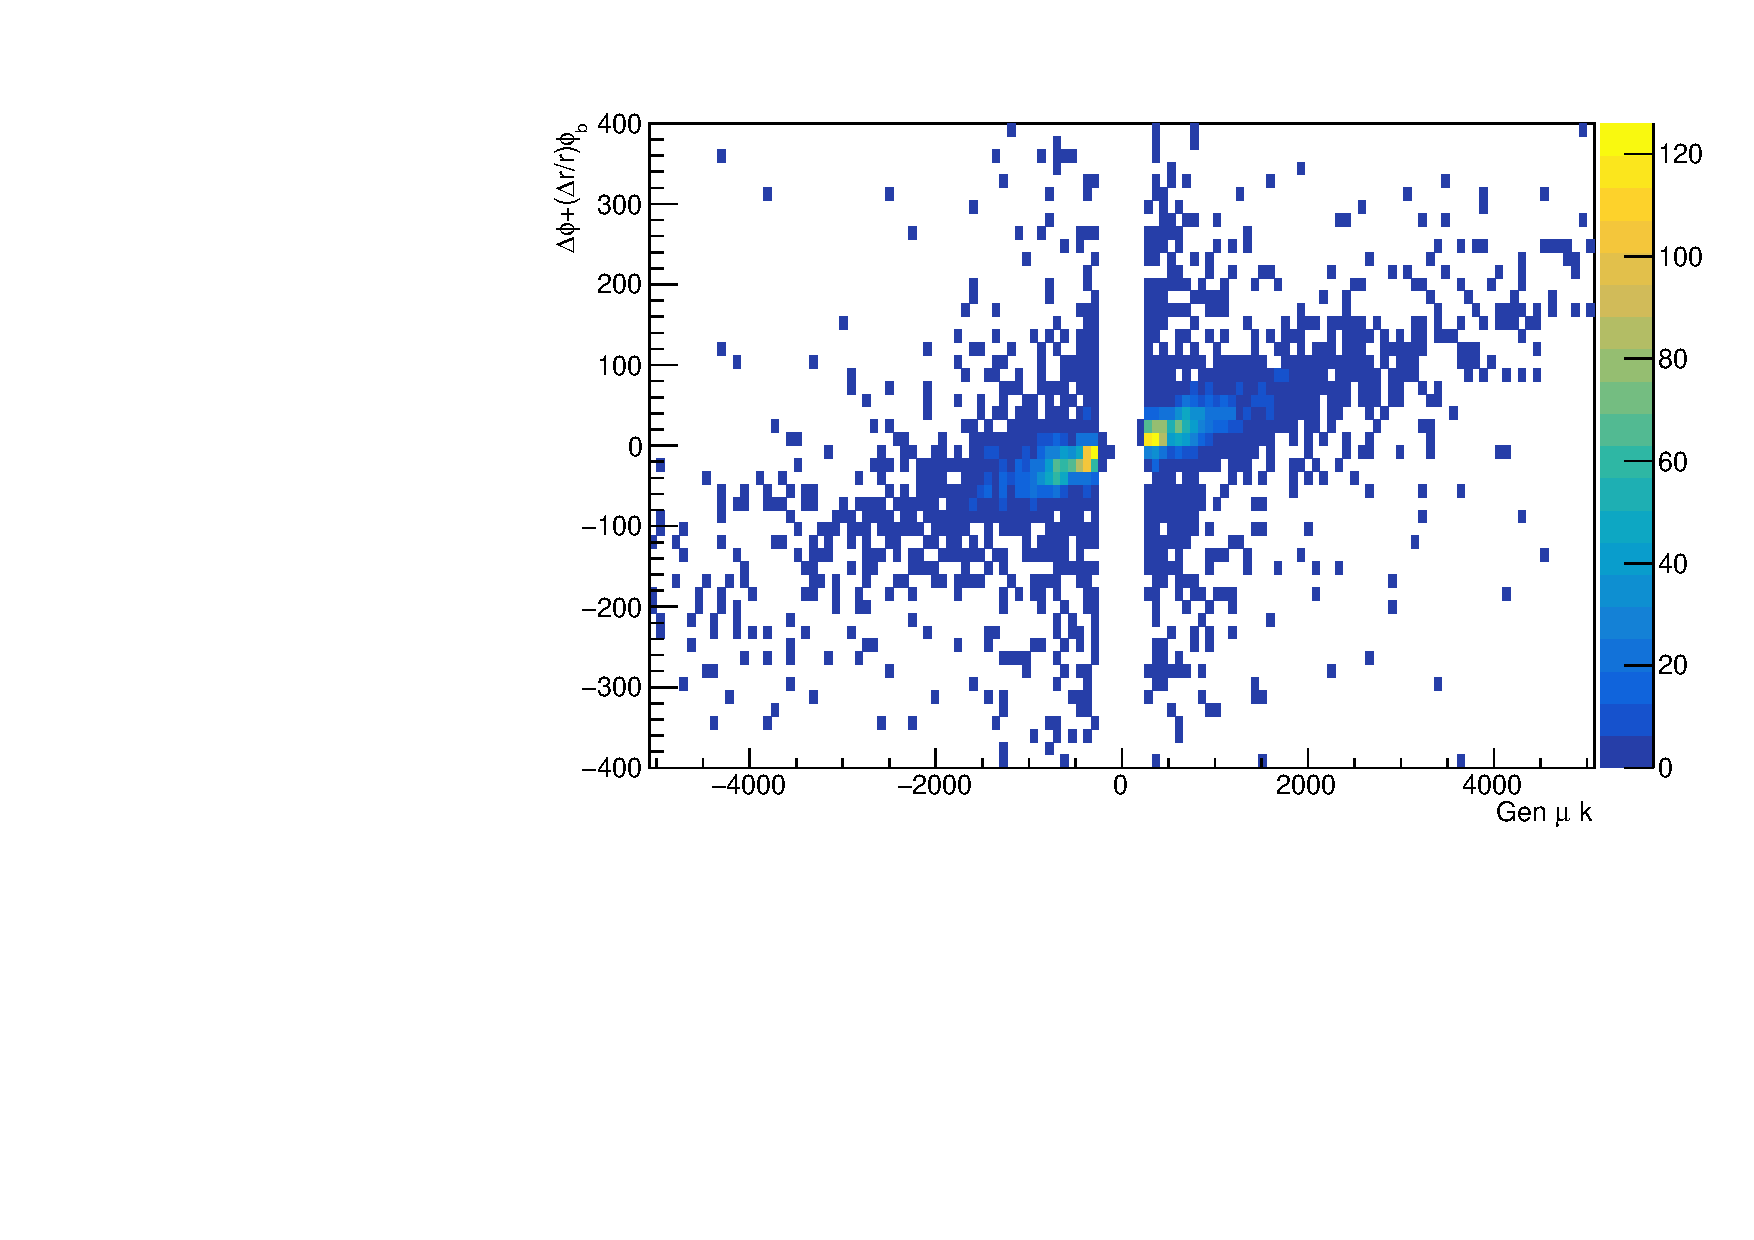
\includegraphics[width=0.32\linewidth]{figs/04_muons/phiprop_2d.pdf}
	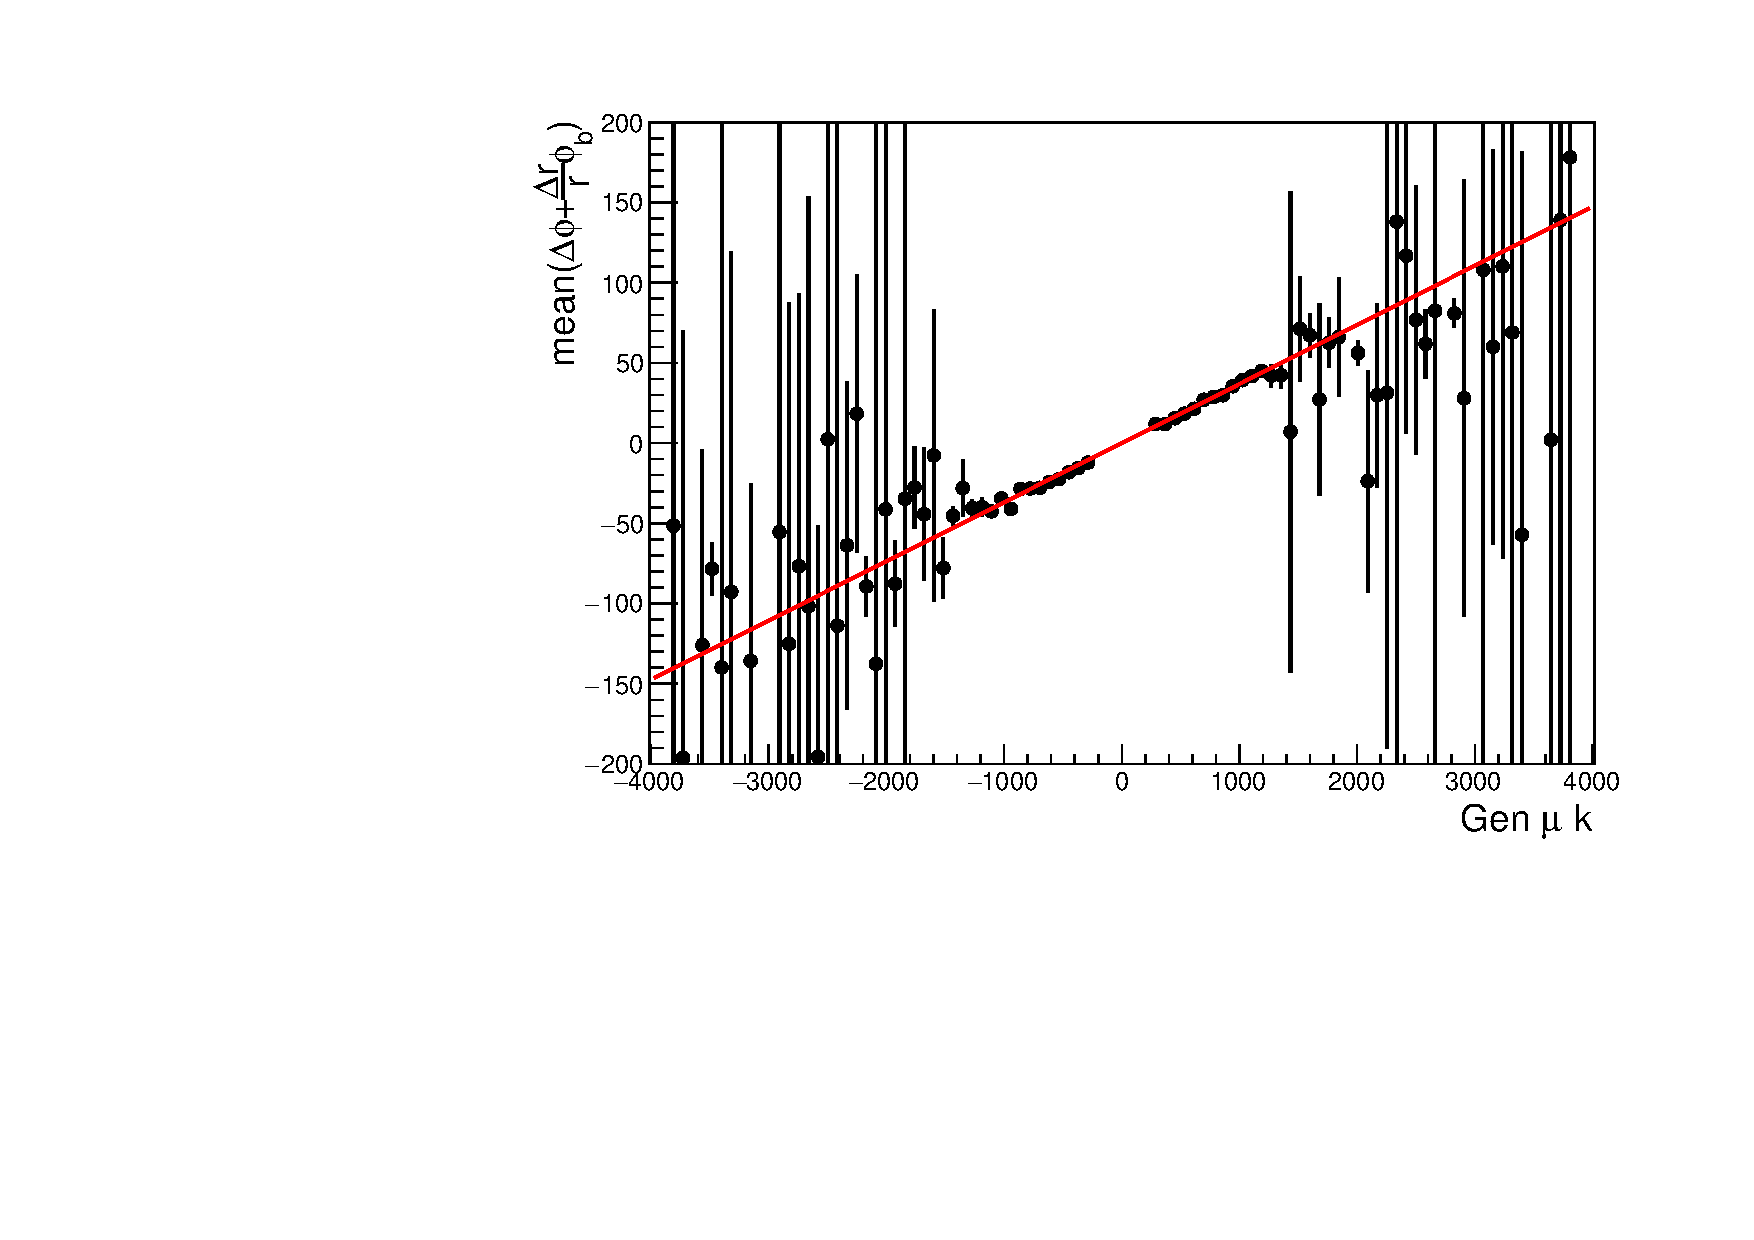
\includegraphics[width=0.32\linewidth]{figs/04_muons/phiprop_mean.pdf}
	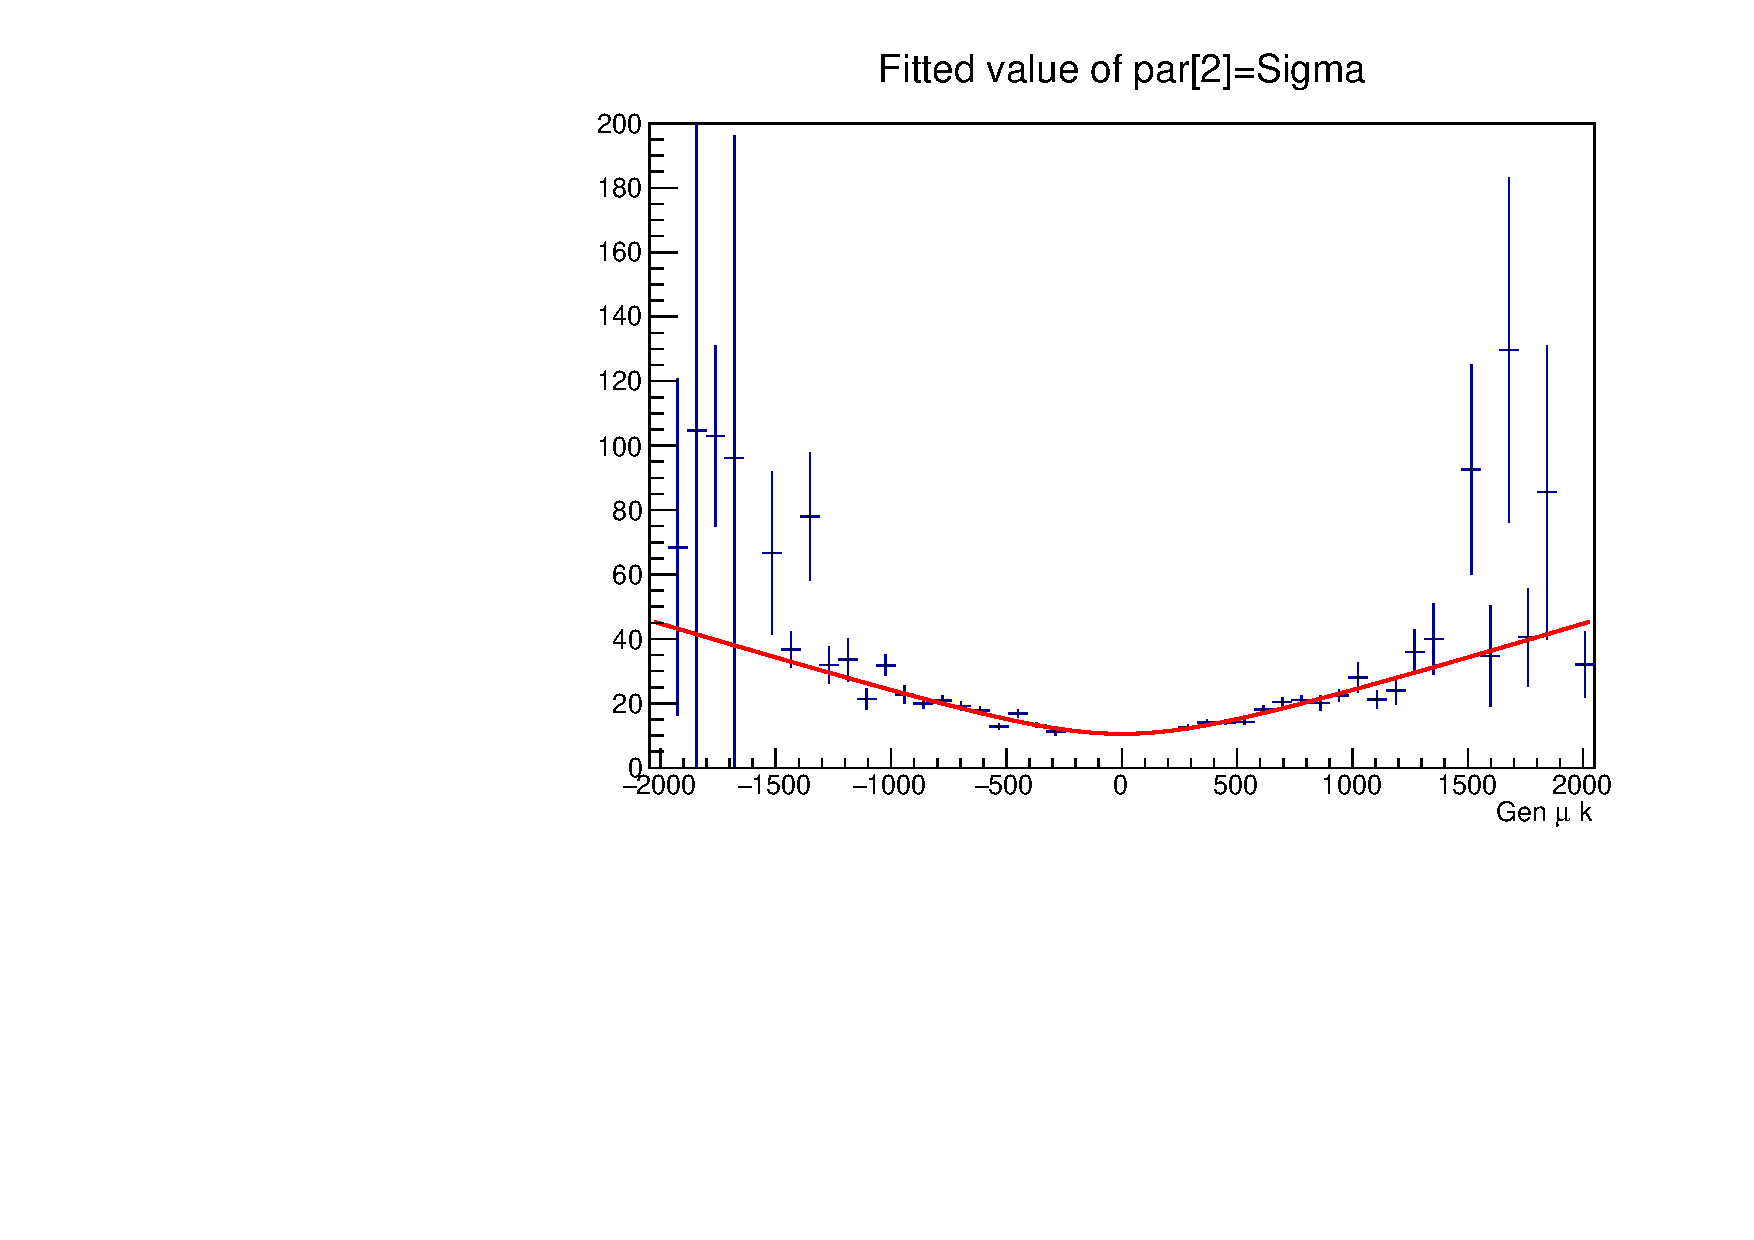
\includegraphics[width=0.32\linewidth]{figs/04_muons/phiprop_sigma.pdf}
	\caption[Calculation of phi propagation coefficients. Units are converted to their digitized form used in firmware calculation. (Left) 2-dimension histogram of $\Delta\phi+\frac{\Delta r}{r_1}\phi_{b,0}$ vs $k$. (Center) Mean of vertical slices fits used to calculate $\alpha$. (Right) Sigma of vertical slices used to calculate multiple scattering and resolution uncertainties.]
	{Calculation of phi propagation coefficients. Units are converted to their digitized form used in firmware calculation. (Left) 2-dimension histogram of $\Delta\phi+\frac{\Delta r}{r_1}\phi_{b,0}$ vs $k$. (Center) Mean of vertical slices fits used to calculate $\alpha$. (Right) Sigma of vertical slices used to calculate multiple scattering and resolution uncertainties.}
	\label{fig:phi_prop}
\end{figure}

Each stub has a measured value representing the "quality" of the hits, with higher values representing a more robust reconstruction of the bending angle. For this reason, the $\phi_b$ position resolutions are calculated separately for high and low quality stubs, as the uncertainty can differ by over a factor of 10 between the two. 

Since the muon detectors only measure $\phi$ and $\phi_b$, the matrix $H$ described in equation~\ref{eq:changeOfBasis} must be a 2$\times$3 matrix that takes the form
\begin{equation}
	H=\left(\begin{matrix}
		0 & 1 & 0\\
		0 & 0 & 1\end{matrix}\right)
\end{equation}

From this, the Kalman Gain $K'$ defined in equation~\ref{eq:gain2} must be a 3x2 matrix with indices $K_{ij}$, and the update step can be explicitly written as
\begin{equation} \label{eq:kmtfUpdate}
	\begin{split}
		k_n^\mathrm{upd}=k_{n-1}+K_{00}\Delta\phi+K_{01}\Delta\phi_b \\
		\phi_n^\mathrm{upd}=\phi_n^\mathrm{prop}+K_{10}\Delta\phi+K_{11}\Delta\phi_b \\
		\phi_{b,n}^\mathrm{upd}=\phi_{b,n}^\mathrm{prop}+K_{20}\Delta\phi+K_{21}\Delta\phi_b
	\end{split}
\end{equation}
where $\Delta\phi$ and $\Delta\phi_b$ are the residuals for $\phi$ and $\phi_b$.

\subsection{Firmware Implementation of the KBMTF} \label{sec:fw}

Two minor approximations are made in order to reduce algorithmic latency and memory usage for firmware implementation. The position resolution of $\phi$ is substantially smaller than the multiple scattering resolution, so the track $\phi$ is set automatically to the measured stub $\phi$. This is equivalent to fixing $K_{10}=1$ and $K_{11}=0$ in equation~\ref{eq:kmtfUpdate}. Secondly, due to the high uncertainty associated with both the measured and propagated $\phi_b$, tracks using three or more stubs set $K_{i1}$ equal to zero and only update using the residual from $\phi$. 

Although the Kalman Gain can can be exactly calculated exactly given the covariance matrices using equation~\ref{eq:gain}, matrix inversion cannot be implemented into the hardware based trigger. In hardware, division is significantly more resource intensive than multiplication, so the calculation of the determinant for matrix inversions would cause the algorithm to exceed the latency requirements for real time track finding. Instead, the values of $K_{ij}$ are stored in look-up tables (LUTS) as a function of curvature and track pattern (the combination of stations that were used to update the track). For tracks with only two stubs, the LUT contains the exact values of the gain that would have been calculated using equation~\ref{eq:gain}. For tracks with more than two stubs, this is an approximation that loses some information from updates at previous stations but produces nearly identical performance.

As outlined in section~\ref{sec:kbmtf_cov}, the $\phi_b$ resolution coefficients are different for high and low quality stubs, thus the values of $K_{i1}$ should depend not only on track pattern and curvature but also the quality of the stubs used to update the track. This would exponentially increase the number of gains stored on LUTs beyond the memory capacity of the hardware. However, from previous approximations, the value of $K_{11}$ is fixed at 0, and $K_{01}$ and $K_{21}$ are only used for two stub tracks. These six track patterns must include gains for the four combinations of outer and inner stub quality.

The firmware is written using Vivado High Level Synthesis (HLS) which compiles firmware written in C to HDL, optimizing it for a given FPGA and clock frequency~\cite{Bachtis:2648953}. When synthesized using the same model and frequency as the BMTF, the KBMTF algorithm can process a single event in 26 clock cycles at 160~\unit{MHz} (equivalent to one every 6.5 bunch crossings), and is pipelined to allow for continuous processing of events. Table~\ref{tab:kmtfFW} shows the resource utilization of the KBMTF compared to the previous BMTF algorithm.

\begin{table} [h!]
	\begin{centering}
	\begin{tabular}{|l|r r r r|}
	\hline
	Algorithm & LUT & FF & BRAM & DSP \\
	\hline
	Phase I BMTF & 43\% & 23\% & 35\% & 0\%\\
	KBMTF & 29\% & 12\% & 20\% & 35\% \\
	\hline 
	\end{tabular}
	\caption[Comparison of FPGA resource utilization. The KBMTF utilizes DSP cores for arithmetic operations to propagate and update tracks and LUTs for the propagation coefficients and approximate Kalman Gain, while the BMTF uses LUTs to assign momentum~\cite{Bachtis:2648953}]
	{Comparison of FPGA resource utilization. The KBMTF utilizes DSP cores for arithmetic operations to propagate and update tracks and LUTs for the propagation coefficients and approximate Kalman Gain, while the BMTF uses LUTs to assign momentum~\cite{Bachtis:2648953}}
	\end{centering}
	\label{tab:kmtfFW}
\end{table}

\section{Performance of the Kalman Barrel Muon Track Finder} \label{sec:kmtf_performance}
The performance of an trigger algorithm is primarily determined by the rate and efficiency. The efficiency is the fraction of signal events that successfully have a track reconstructed by the algorithm, while the rate is the frequency that the algorithm will trigger. A high efficiency is desirable to ensure any interesting events are stored for future analysis, while a low rate is crucial to reject background events and provide a reasonable bandwidth to write events to tape. This section will compare the relative performances of the previous algorithm with the KBMTF.

\subsection{Trigger Efficiencies} \label{sec:kmtf_eff}
The previous L1 barrel muon trigger (BMTF) functioned by using pairs of stubs to form tracks, then using a LUT to assign track parameters based on the $\phi$ and $\phi_b$ of the stubs. This LUT takes only the $\phi$ and $\phi_b$ of the two stubs and was calculated with the assumption that the muon originated from the beamspot. In the case of displaced muons, which arise from secondary decays of long lived exotic, beyond standard model particles, the assumption is no longer valid and results in large inefficiencies as the muon becomes more displaced from the beamspot.

The general efficiency of a trigger is defined as the fraction of signal muons that have a matching reconstructed track, and can be expressed abstractly as

\begin{equation}\label{eq:eff}
	\epsilon=\frac{N_\mathrm{signal}(\mathrm{Passing\ trigger})}{N_\mathrm{signal}}	
\end{equation}

For muon triggers, the denominator of signal muons consist of events that have known information about the muons. This can be from generator information in simulated monte-carlo samples, tracker information using cosmic muon data, or probe muons using the tag-and-probe method on data. These signal muons are cut using the known muon information to produce a reasonable sample for track reconstruction. For example, the denominator for barrel muon algorithms would not contain very forward muons in the endcap at high $|\eta|$. The numerator consists of signal muons with a matching reconstructed track that may have addition cuts on the reconstructed track properties.

Figure~\ref{fig:effVsDxy_kmtf} shows the efficiency versus muon $d_{xy}$ for three track finding algorithms. The denominator consists of cosmic ray muons passing through the barrel muon detectors with a $p_T>20\unit{GeV}$. The numerator requires a matching L1 track with reconstructed $p_T>10\unit{GeV}$. The first algorithm is the BMTF, which shows inefficiencies due to the $p_T$ LUTs assuming the muon originated at the beamspot. The second is the prompt KBMTF, which uses the vertex constrained measurement. This also shows inefficiencies due to the vertex constraint, but is better than the BMTF as the vertex constraint isn't applied until the last step of track reconstruction. Lastly, the displaced KBMTF uses the vertex unconstrained measurement and shows substantial improvements compared to both prompt algorithms.

\begin{figure}[htbp!]
	\centering
	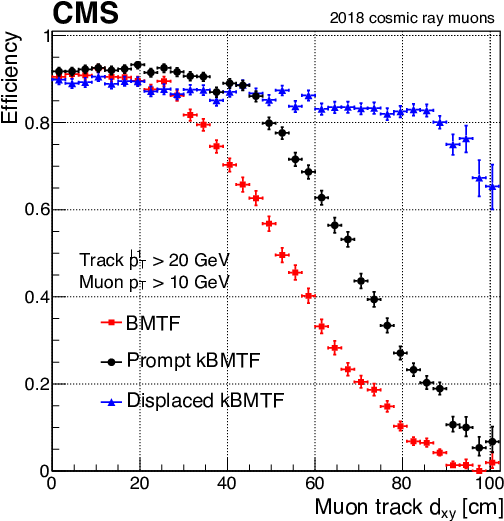
\includegraphics[width=0.55\linewidth]{figs/04_muons/effVsDxy_kmtf.png}
	\caption[Comparison of efficiency vs cosmic track $l_{xy}$ using cosmic data from the 2018 data taking run. The prompt KBMTF takes the reconstructed $p_{T}$ using the vertex constrained measurement, while the displaced KBMTF uses the veretx unconstrained measurement. The displaced KBMTF shows substantial improvements to the previous BMTF~\cite{cmscollaboration2023development}]
	{Comparison of efficiency vs cosmic track $l_{xy}$ using cosmic data from the 2018 data taking run. The prompt KBMTF takes the reconstructed $p_{T}$ using the vertex constrained measurement, while the displaced KBMTF uses the veretx unconstrained measurement. The displaced KBMTF shows substantial improvements to the previous BMTF~\cite{cmscollaboration2023development}}
	\label{fig:effVsDxy_kmtf}
\end{figure}

\subsection{Firmware and Emulator Agreement} \label{sec:kmtf_fwVsEmu}

The performance of the KBMTF is tested using a dedicated software emulator which is integrated into the CMS analysis framework. This emulator follows similar logic to the HLS code, but is not a one-to-one replica. Several modifications are made to the HLS code in order to make it compatible with the synthesis into HDL and pipelining. As such, a test bench is used to ensure that the output of the firmware and emulator are identical. The emulator runs the algorithm over several events and outputs a text file containing information on the input stubs and the reconstructed tracks. This text file is used as input for the test bench, which  runs the stub information through the HLS code and compares the reconstructed tracks to those found in the emulator.

Disagreements between the emulator and firmware are used for a variety of debugging purposes. They frequently point to logic errors in the simplification of the algorithm for HLS synthesis, or in some cases show bugs in the emulator. Prior to 2020, the disagreements were almost entirely due to differences resulting from fixed point calculations in the firmware compared to floating point calculations in the emulator. These differences have been drastically reduced due to the addition of fixed point calculations in the emulator, which now has a $>$99.9\% agreement.

\begin{figure} [htb!]
	\centering
	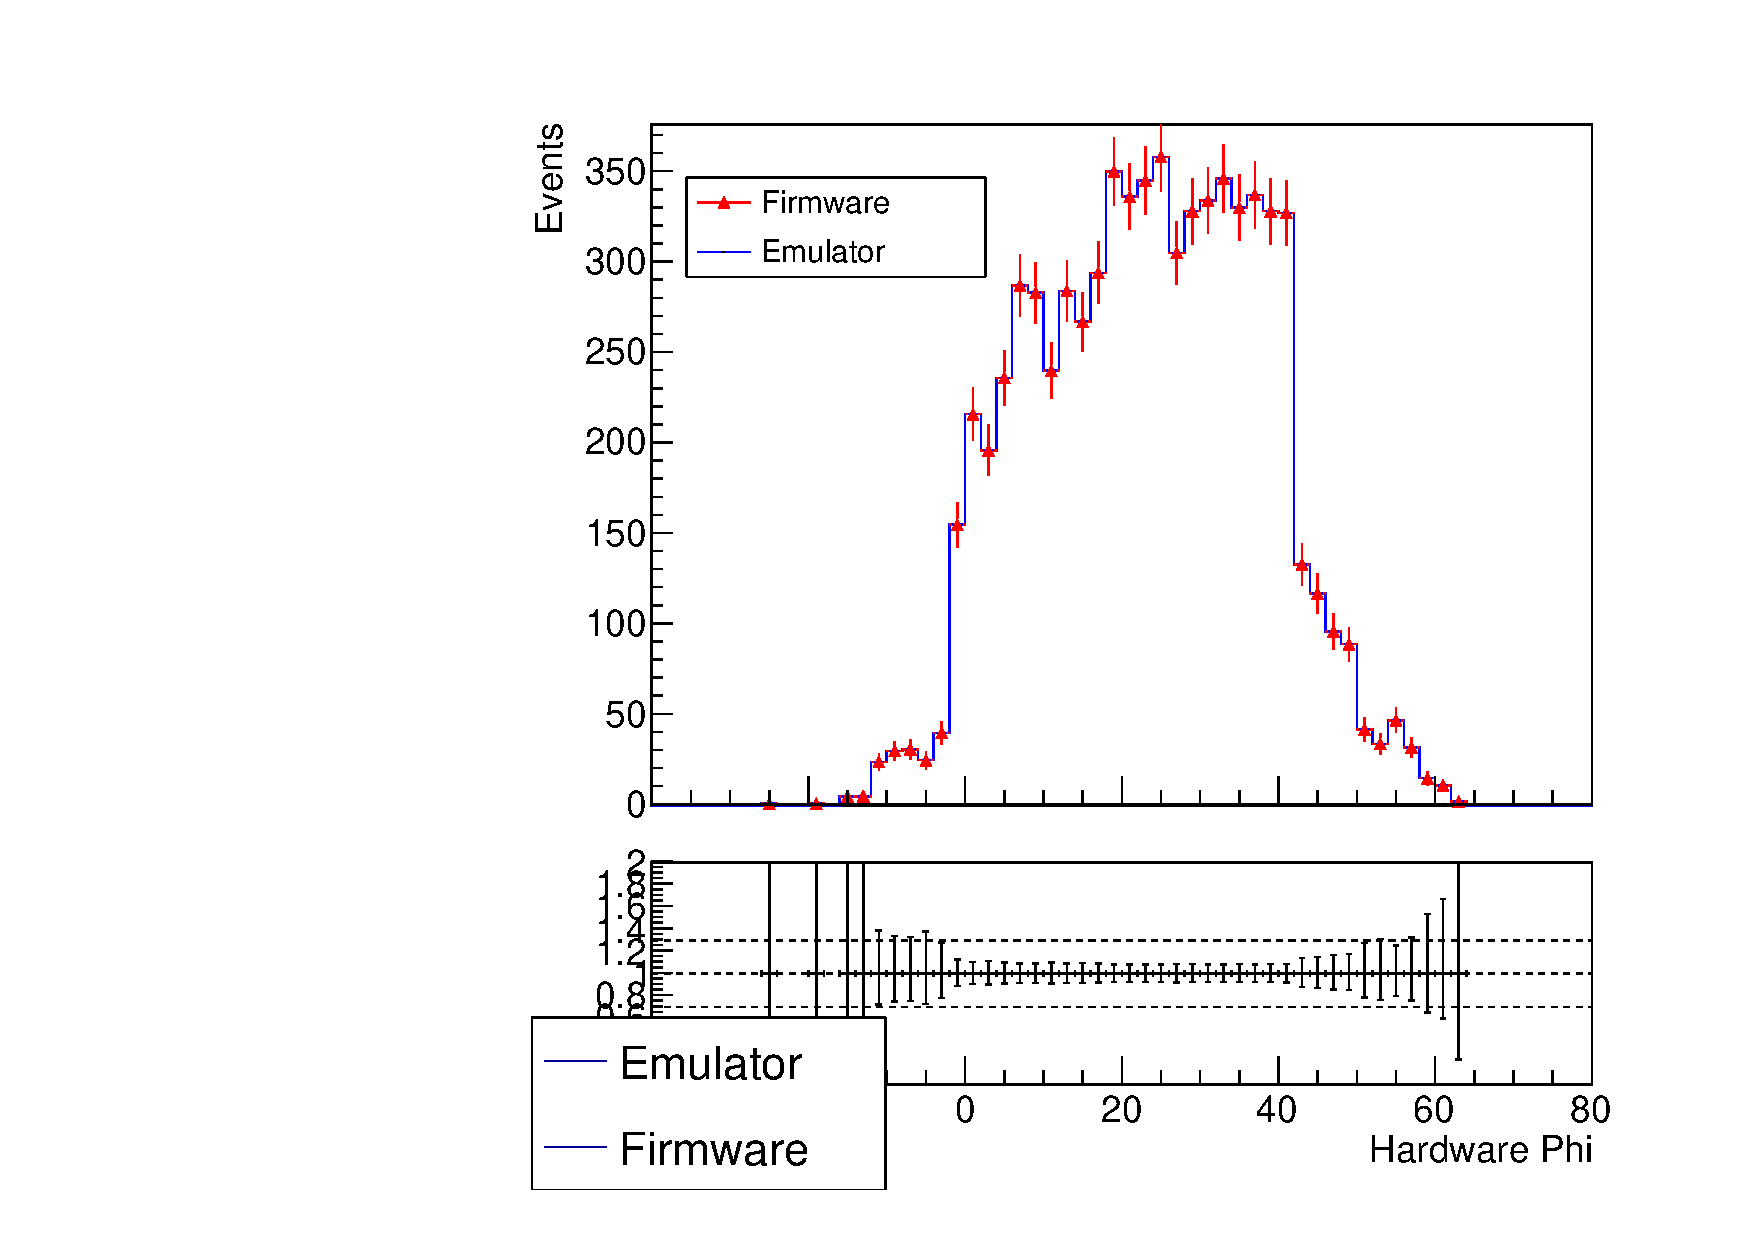
\includegraphics[width=0.75\linewidth]{figs/04_muons/fwVsEmu_phi.pdf}
	\caption[Comparison of the track $\phi$ between the firmware and emulator using data from a 2017 Z tag-and-probe sample. The emulator and firmware output show 100\% agreement across 500000 events.]{Comparison of the track $\phi$ between the firmware and emulator using data from a 2017 Z tag-and-probe sample. The emulator and firmware output show 100\% agreement across 500000 events.}
	\label{fig:kmtf_fwVsEmu}
\end{figure}